\subsection{Results and discussion}


%%%%%%%%%%%%%%%%%%%%%%%%%%%%%%%%%%%%%%%%%%%%%%%%%%%%%%%%%%%%%%%%
%%  Systematic quant. of the relationship between stereo. and small molecule bioactivity
%%%%%%%%%%%%%%%%%%%%%%%%%%%%%%%%%%%%%%%%%%%%%%%%%%%%%%%%%%%%%%%%

\phantomsection
\subsubsection{Systematic quantification of the relationship between stereochemistry and small molecule bioactivity}
\label{Stereoisomers_Rel_Stereo_Bioactivity}


The first steps in the development of Signaturizers3D were (i) to select a comprehensive database containing detailed bioactivity data for a wide range of chemical compounds, and (ii) within this database, systematically identify groups of stereoisomers to compare their bioactivity profiles and evaluate the ability of Signaturizers3D to distinguish them.
To gather bioactivity data, we used the Chemical Checker (CC), which represents the largest collection of small molecule bioactivity signatures available to date, with experimental information for over 1M compounds\cite{duran-frigola_extending_2020}. \hl{The CC divides data into five levels of increasing complexity, ranging from the chemical properties of compounds to their clinical outcomes. Compound bioactivities are expressed in a vector-like format (i.e. signatures), and the data processing pipeline also includes several steps of increasing level of integration and abstraction: from raw experimental data representing explicit knowledge (type 0 signatures) to inferred representations that leverage all the experimentally determined bioactivities available for each molecule (type III signatures).} Thus, we processed the whole CC (i.e. 25 different bioactivity types for about 1M molecules) to systematically identify groups of stereoisomers that might exhibit distinct bioactivities. In brief, we first identified stereoisomers using their InChIKey strings and we then applied several filters to ensure that the actual differences between compounds were exclusively due to stereochemical variations (see \hyperref[Stereoisomers_Methods]{Methods} for further details). Then, we selectively removed molecules that were not exhaustively characterized, in order to work with enantiomerically pure compounds and prevent the analysis of results derived from racemic mixtures (Fig \ref{Stereoisomers_Fig1}a). We eventually identified 23,830 groups of stereoisomers, involving 57,989 compounds, across the different CC bioactivity spaces. We found most stereoisomeric groups with experimental information in the target binding space (B4) and in the network spaces derived from B4 (i.e. C3-5, Fig \ref{Stereoisomers_FigS1}). We thus focused our study on the B4 space, which contains over 600,000 molecules, and we identified 15,370 groups of stereoisomers, involving 32,705 compounds (Fig \ref{Stereoisomers_Fig1}b). We then analyzed the binding profiles for all these compounds, and found 6,022 groups that had at least 2 stereoisomers with non-identical binding profiles. We also observed that the majority of the groups (14,181, \textasciitilde92\%) contained only 2 stereoisomers (Fig \ref{Stereoisomers_Fig1}c, top), in 38\% of which both compounds showed distinct binding profiles (Fig \ref{Stereoisomers_Fig1}c, bottom). Analogously, we identified 562 groups containing 3 stereoisomers: 230 (41\%), 195 (35\%) and 137 (24\%) of them showing 1, 2 and 3 distinct binding profiles, respectively. Finally, we observed that the distribution of Jaccard distances between binding profiles within stereoisomeric groups was skewed towards low values (i.e. more similar profiles) compared with random pairs, while pairs of compounds sharing at least one target were somewhere in the middle (Fig \ref{Stereoisomers_Fig1}d). Fig \ref{Stereoisomers_Fig1}e shows, as an illustrative example, a group of 3 stereoisomers with non-identical binding profiles, where compounds A and C weakly and strongly bind with the Beta-1 adrenergic receptor (ADRB1; 2\textsuperscript{nd} position in the profile), respectively, whilst compound B does not bind it. Note that inactive compound-target interactions might be false negatives due to, for instance, a limited sensitivity of the detection methods or non-tested enantiomers.


\begin{Figure_modified}
  \centering
  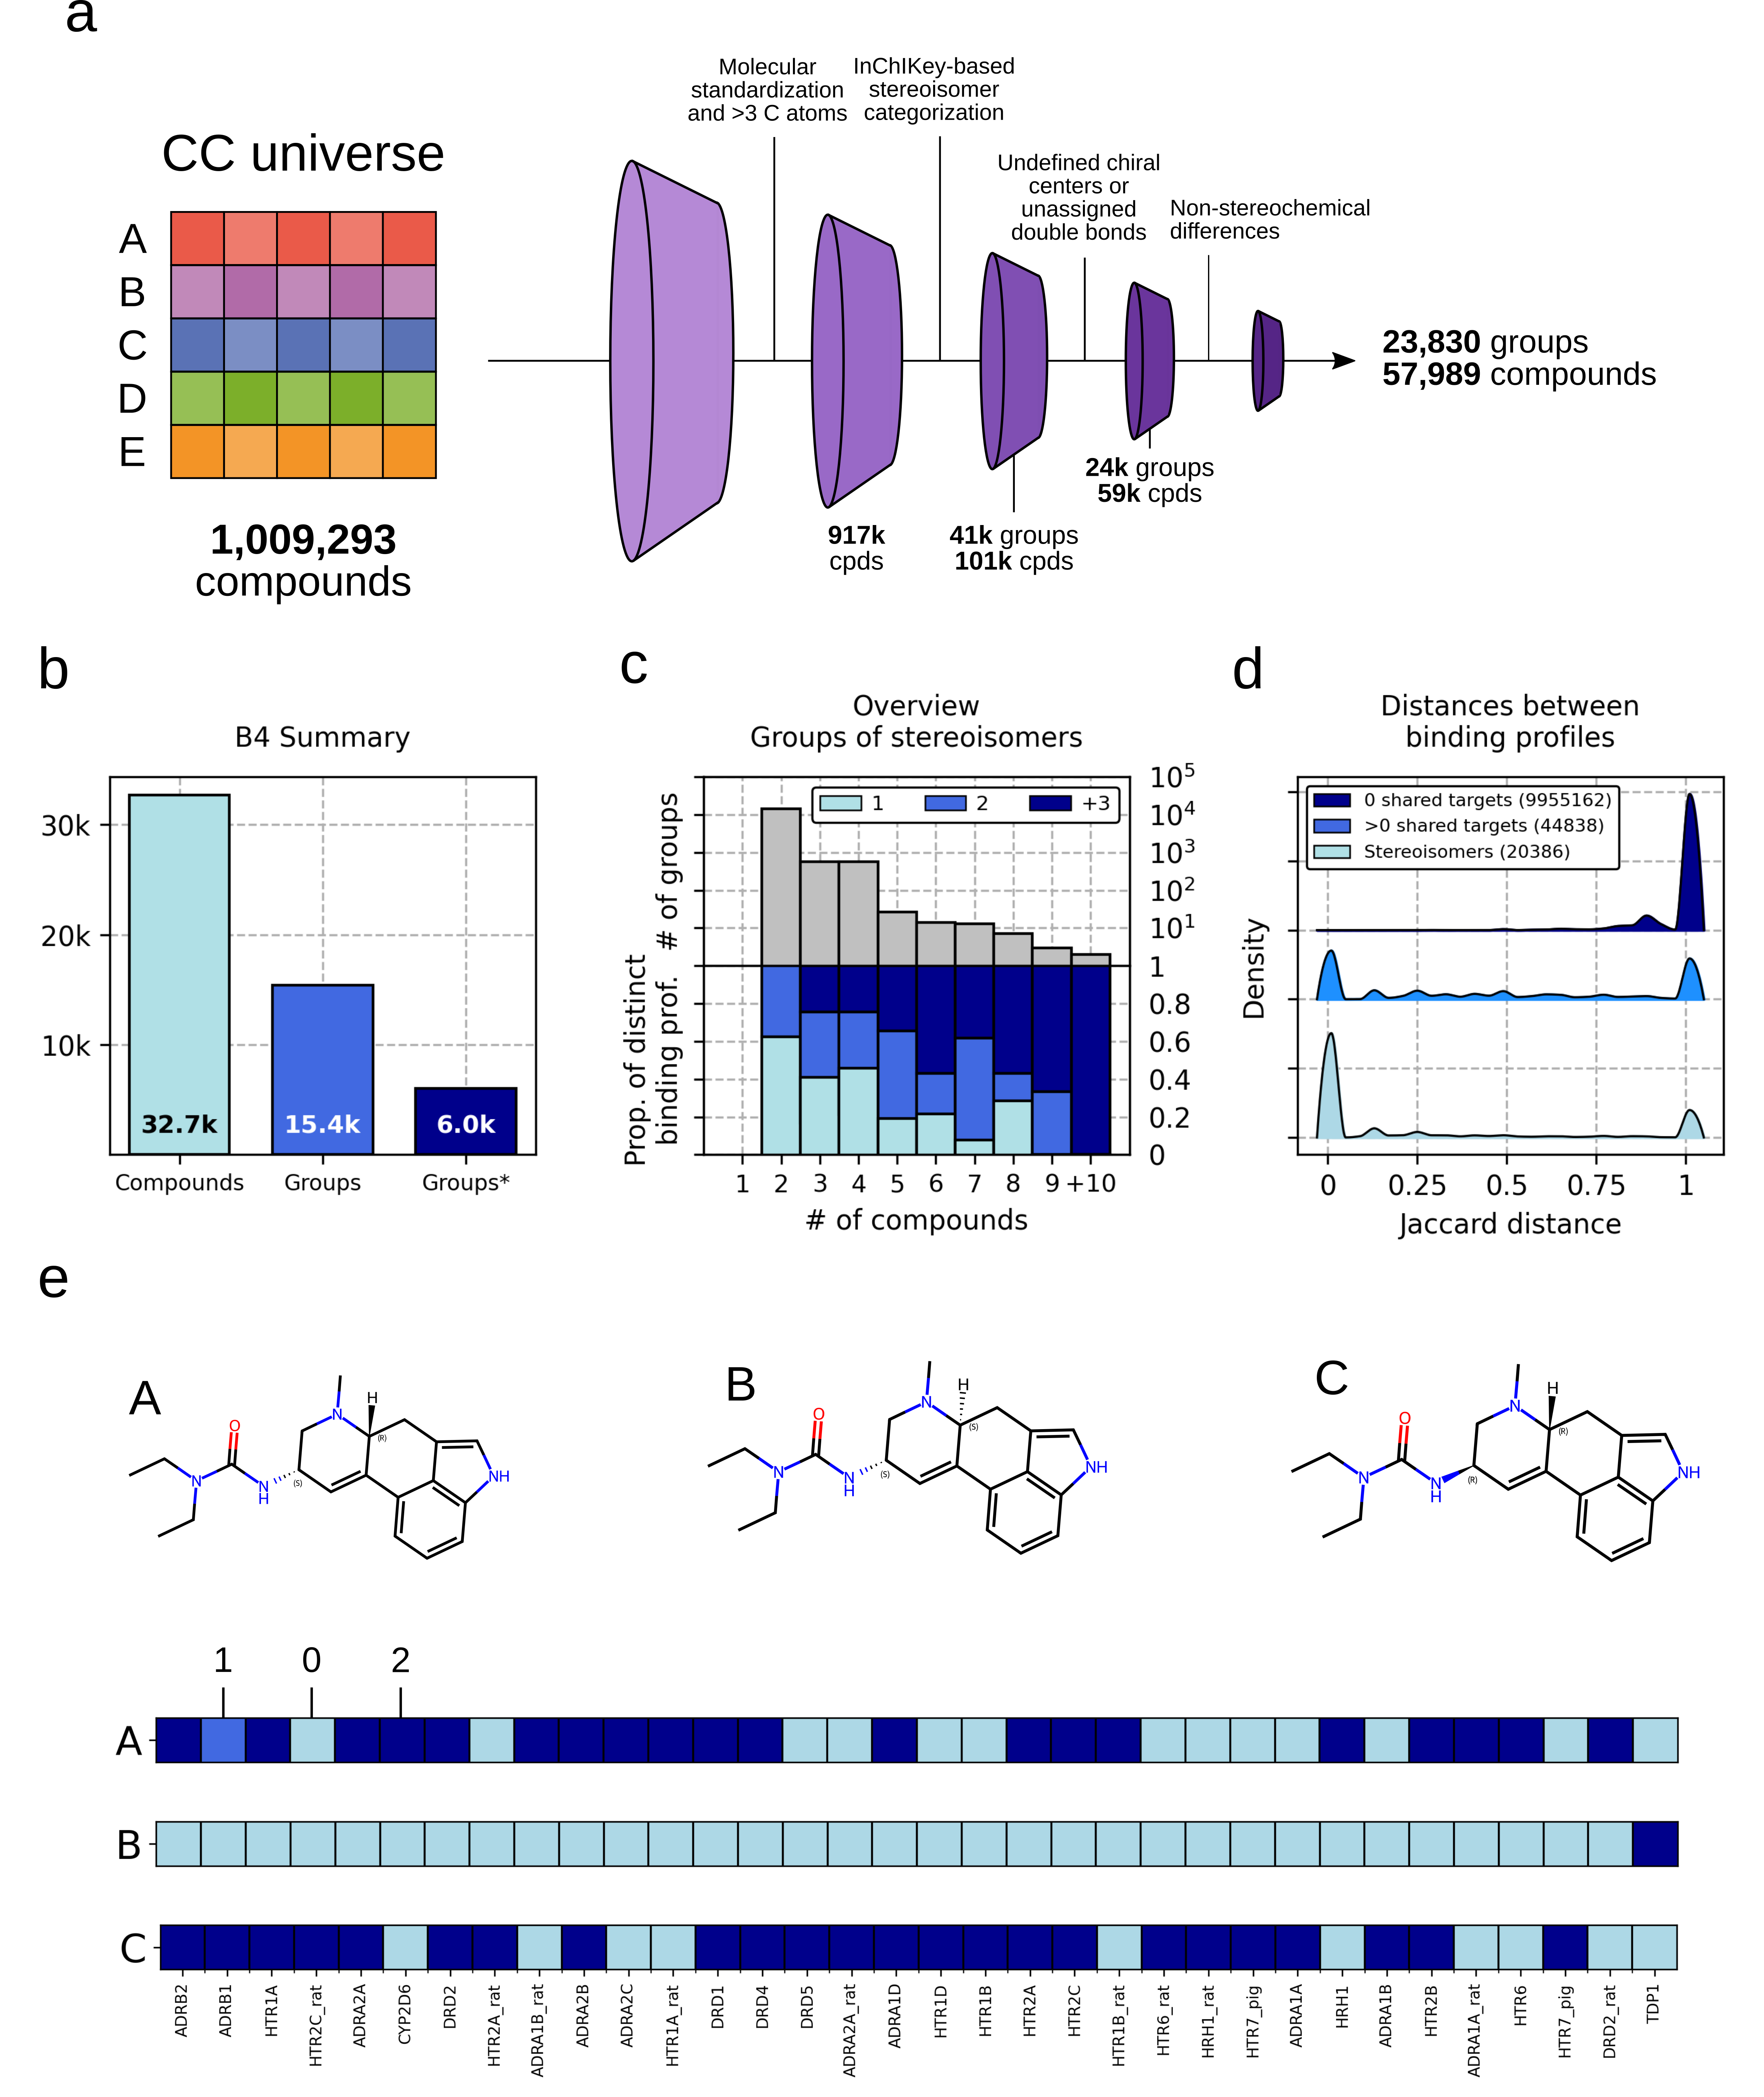
\includegraphics[width=1\linewidth]{figures/Stereoisomers/Main/Fig1_v2.png}
  \caption{
    \textbf{Stereoisomerism and bioactivity.}
    \textbf{a)} Computational pipeline to identify groups of stereoisomers in the CC chemical universe.
    \textbf{b)} Number of unique stereoisomeric compounds with experimentally identified protein targets in the CC B4 space, number of stereoisomer groups, and number of groups with at least 2 compounds with non-identical binding profiles.
    \textbf{c)} Number of groups (y-axis, top) having the specified number of stereoisomers (x-axis). Proportion of these groups (y-axis, bottom) having the specified number of distinct binding profiles (i.e. \textasciitilde60\% of the groups of 2 isomers have a unique binding profile).
    \textbf{d)} Distributions of Jaccard distances (binding profiles) between pairs of compounds sharing 0, ≥1 targets and stereoisomer pairs. All distributions are significantly different from each other (Mann-Whitney p-value\textasciitilde0).
    \textbf{e)} Illustrative example of a stereoisomer group including 3 small molecules with their corresponding target binding profiles, using the annotation of type 0 signatures (i.e. 0: no binding; 1: weak binding and 2: strong binding).
    \rule[0ex]{\textwidth}{0.5pt}
  }
  \label{Stereoisomers_Fig1}
\end{Figure_modified}


%%%%%%%%%%%%%%%%%%%%%%%%%%%%%%%%%%%%%%%%%%%%%%%%%%%%%%%%%%%%%%%%
%%  Design and evaluation of stereochemically-aware Signaturizers
%%%%%%%%%%%%%%%%%%%%%%%%%%%%%%%%%%%%%%%%%%%%%%%%%%%%%%%%%%%%%%%%

\phantomsection
\subsubsection{Design and evaluation of stereochemically-aware Signaturizers}
\label{Stereoisomers_Design_Evaluation_Signaturizers}

Our analyses showed that most stereoisomer pairs (60.4\%) had identical target profiles but, perhaps more interestingly, the remaining 8,081 pairs (39,6\%) showed distinct binding against protein targets (Fig \ref{Stereoisomers_Fig2}a). We also observed that CC type III signatures captured differences between stereoisomer pairs (Fig \ref{Stereoisomers_Fig2}b). However, these differences were fully missed by the Signaturizers (Fig \ref{Stereoisomers_Fig2}c), as they were trained on 2D representations of the chemical molecules (i.e. ECFP4\cite{rogers_extended-connectivity_2010}), highlighting the need to develop new descriptors able to distinguish stereoisomer-specific bioactivities.

To overcome the limitations of the original Signaturizers, we trained new deep-networks using 3D-aware molecular representations (i.e. Signaturizers3D, Fig \ref{Stereoisomers_Fig2}e). We first generated 3D conformations for all CC molecules, coupled them with their type III signatures, and used them to fine-tune the pre-trained Uni-Mol model\cite{zhou_uni-mol_2023}. In brief, for all molecules in the CC, we generated and optimized a single 3D conformation per compound using the ETKDG method\cite{riniker_better_2015} and the Merck Molecular Force Field (MMFF94) from RDKit. After removing hydrogens, all coordinates and atom-types for each molecule were used to fine-tune the pre-trained Uni-Mol model as a multitarget regression problem, so that we could directly infer pre-calculated CC type III signatures (128 dimensions). Specific details regarding the training of the models are provided in the Supplementary Information. We then evaluated the capability of Signaturizers3D to distinguish stereoisomers by generating B4 signatures for the 32,705 compounds identified as stereoisomers in the CC B4 space and calculating distances between them. We found that, opposed to the original Signaturizers, virtually all pairs of stereoisomers (99.9\%) exhibited non-identical 3D signatures (Fig \ref{Stereoisomers_Fig2}f), showcasing the ability of our new models to capture slight differences in the stereochemistry of the compounds. Next, we followed a strict approach to assess the ability of Signaturizers3D to recapitulate k-nearest neighbor (kNN) compounds at type III signature level; this is to evaluate their capacity to retain the structure of the original data similarity. In brief, in a standard kNN recovery task, negative pairs are chosen randomly and can differ significantly from positive pairs (Fig \ref{Stereoisomers_FigS2}a). We used the same strategy to evaluate the capacity of the new descriptors to retain traceable biological information (e.g. type 0 signatures), in the form of compound-target pairs (Fig \ref{Stereoisomers_FigS2}b). Under this scenario, both Signaturizers and Signaturizers3D could almost perfectly distinguish close from distant molecules at type III and 0 signatures level. To make the assessment more stringent and realistic, we selected the negatives within a close distance of the molecule under evaluation, making the discernment between positive and negative pairs a more difficult task (Fig \ref{Stereoisomers_FigS2}c; see \hyperref[Stereoisomers_Methods]{Methods}). In this case, we observed that, indeed, Signaturizers3D were able to better recapitulate type III and 0 signatures than the original ECFP4-based Signaturizers (Fig \ref{Stereoisomers_Fig2}g, h).


\begin{Figure_modified}
  \centering
  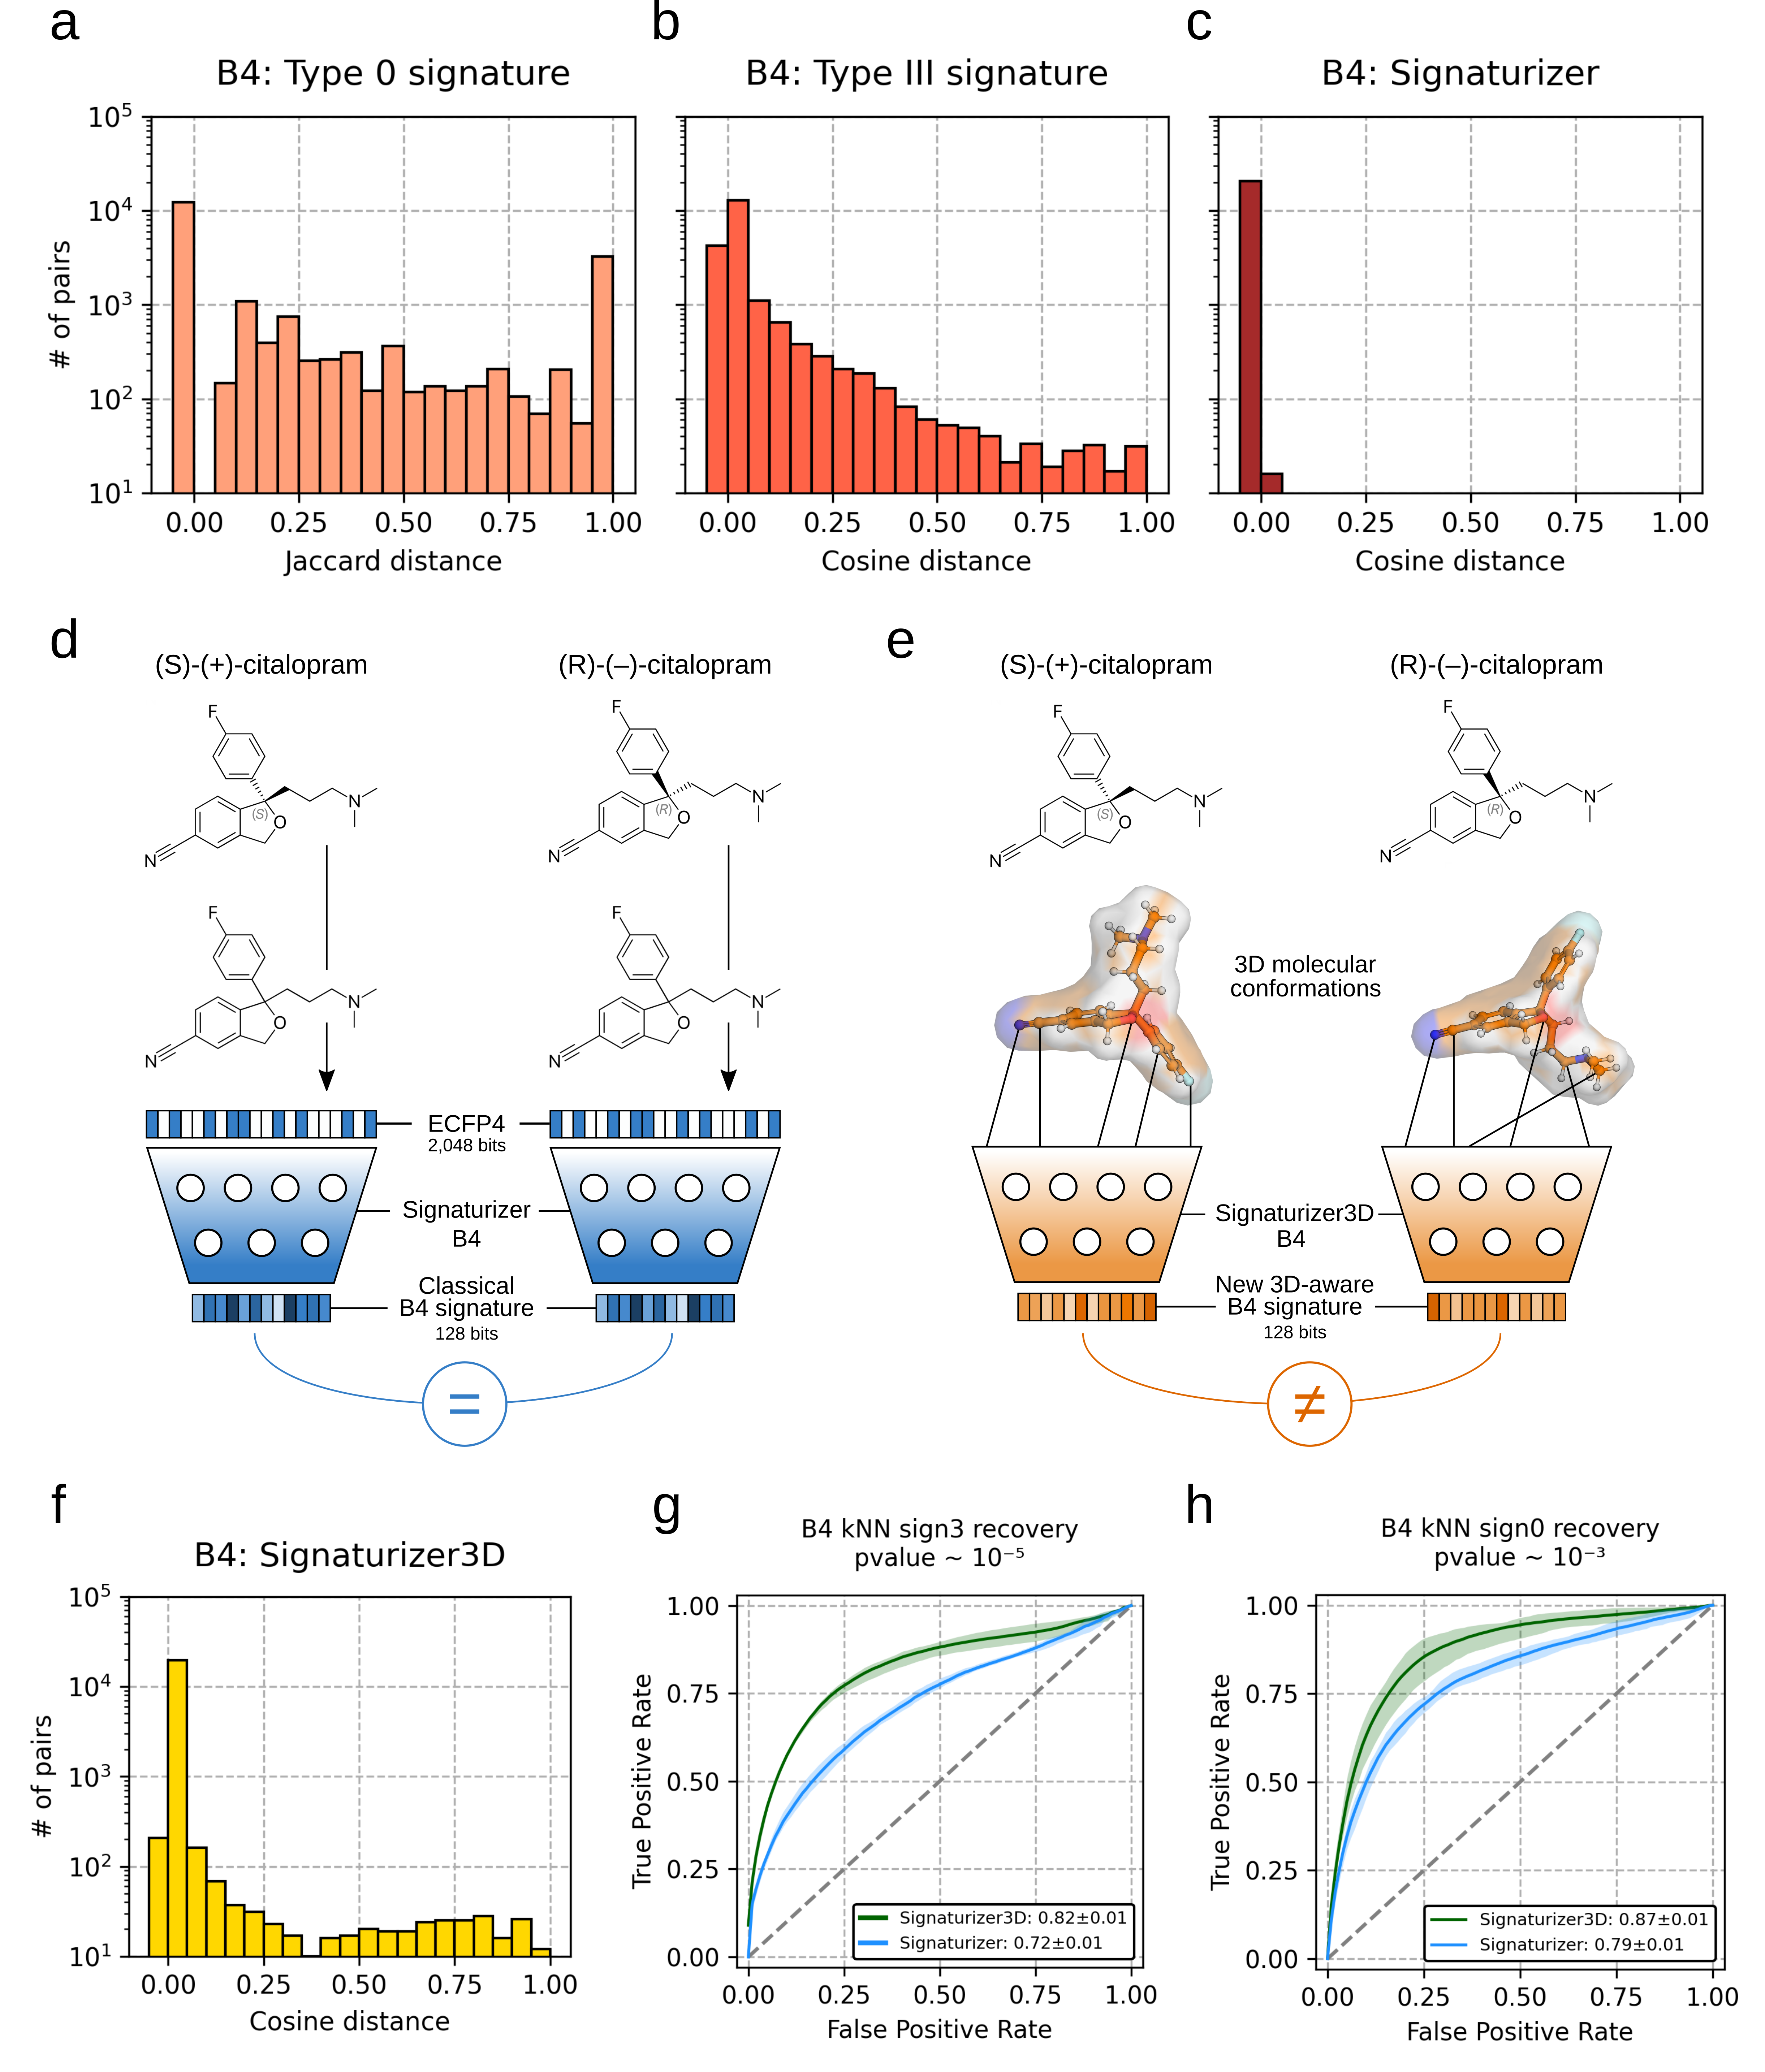
\includegraphics[width=1\linewidth]{figures/Stereoisomers/Main/Fig2_v4.png}
  \caption{
    \textbf{Stereochemically-aware bioactivity descriptors.}
    \textbf{a)} Distribution of target binding profile Jaccard distances (CC B4 type 0 signatures) between stereoisomer pairs (20,386 pairs).
    \textbf{b)} Distribution of CC B4 type III signature cosine distances between stereoisomer pairs.
    \textbf{c)} Distribution of Signaturizer cosine distances between stereoisomer pairs.
    \textbf{d)} Graphical scheme of the \textit{signaturization} process of distinct stereoisomers ((S)-(+)-citalopram and (R)-(–)-citalopram) with the Signaturizer. Molecules are first represented by 2D-based fingerprints (ECFP4, 3D information is lost) and then input to a neural network. Since ECFP4 for both stereoisomers are identical, output signatures are also identical.
     \textbf{e)} Graphical scheme of the signaturization process of distinct stereoisomers ((S)-(+)-citalopram and (R)-(–)-citalopram) with the novel Signaturizer3D. 3D conformations are first generated for both molecules and the corresponding molecular representations are input to the Signaturizer3D fine-tuned neural network. Since molecular representations for both stereoisomers are different, output signatures are also different.
     \textbf{f)} Distribution of Signaturizer3D cosine distances between stereoisomer pairs.
     \textbf{g)} Recapitulation of B4 signature type III kNNs (x3 80/20 splits) using the original Signaturizer and the Signaturizer3D. Nearest neighbors are defined as those molecules with a B4 cosine distance to the evaluated compound in the 0.001 percentile of the distribution (p-value \textasciitilde10\textsuperscript{-5}).
     \textbf{h)} Recapitulation of B4 signature type 0 kNNs using the original Signaturizer and the Signaturizer3D. Nearest neighbors are defined as those molecules with a B4 cosine distance to the evaluated compound in the 0.1 percentile of the distribution (p-value \textasciitilde10\textsuperscript{-3}). To speed up the comparisons, positive (NN) and negative (non-NN) pairs were subsampled (10x2.5k compounds) from the CC B4 space.
    \rule[0ex]{\textwidth}{0.5pt}
  }
  \label{Stereoisomers_Fig2}
\end{Figure_modified}